\documentclass[12pt]{report}

\usepackage[titletoc]{appendix}
\usepackage{datetime}
\usepackage{graphicx}
\usepackage{amsmath}
\usepackage{algorithmicx}
\usepackage{algorithm}
\usepackage[explicit]{titlesec}
\usepackage{tocloft}
\usepackage{amssymb}
\usepackage{longtable}
\usepackage{multirow}
\usepackage[english]{babel}

\usepackage{subcaption}
\usepackage{subfig}

\usepackage{url}

\usepackage{rotating}

\renewcommand{\familydefault}{\rmdefault}
\renewcommand\cftchapaftersnum{.}
\renewcommand\cftchapdotsep{\cftdotsep}

\setlength{\textheight}{8.63in}
\setlength{\textwidth}{5.9in}
\setlength{\topmargin}{-0.2in}
\setlength{\oddsidemargin}{0.3in}
\setlength{\evensidemargin}{0.3in}
\setlength{\headsep}{0.0in}

\titleformat{\chapter}[block]
  {\Large\filcenter\bfseries}{\MakeUppercase{Chapter \thechapter}\\}{0em}{\MakeUppercase{#1}}
  
\titleformat{\section}[block]
  {\large\bfseries}{\thesection}{0.5em}{#1}
  
\titleformat{\subsection}[block]
  {\normalsize\bfseries}{\thesubsection}{0.5em}{#1}
  

\newcommand{\signature}{\rule{3in}{1.2pt}}
\newcommand{\thesistitle}{Affective Motivational Collaboration Theory}
\newdateformat{monthyear}{\monthname[\THEMONTH] \THEYEAR}

\DeclareMathOperator*{\argmin}{\arg\!\min}
\DeclareMathOperator*{\argmax}{\arg\!\max}

\linespread{1.5}

\begin{document}

\begin{titlepage}
\begin{center}
\large\textbf{\thesistitle}\\[0.5em]

\large\textnormal{by}\\
\large\textnormal{Mahni Shayganfar - mshayganfar@wpi.edu}\\[0.5em]

\large\textnormal{A PhD Dissertation}\\[0.5em]

\large\textnormal{Presented at}\\[0.5em]
\large\textsc{WORCESTER POLYTECHNIC INSTITUTE}\\[0.5em]
\large\textnormal{in partial fulfillment of the requirements for the}\\[0.5em]
\large\textnormal{DOCTOR OF PHILOSOPHY}\\[0.5em]
\large\textnormal{in}\\
\large\textnormal{Computer Science}\\
\large\textnormal{November 2016}\\[0.75em]
\end{center}

\noindent\large\textsc{Approved}\\[0.5em]
\Large\textnormal{\signature}\\
\normalsize\textnormal{Professor Charles Rich, Thesis Advisor}\\[0.5em]
\Large\textnormal{\signature}\\
\normalsize\textnormal{Professor Candace L. Sidner, Thesis Co-Advisor}\\[0.5em]
\Large\textnormal{\signature}\\
\normalsize\textnormal{Professor John E. Laird, Thesis Committee
Member}\\[0.5em] \Large\textnormal{\signature}\\
\normalsize\textnormal{Professor Stacy Marsella, Thesis Committee Member}
\end{titlepage}

\thispagestyle{empty}
\vspace*{\fill}
  \begin{center}
    \textcopyright \hspace{0.5em} Copyright by Mahni Shayganfar 2016

    All Rights Reserved
  \end{center}
\vspace*{\fill}
\newpage

\pagenumbering{roman}

\chapter*{Abstract}
\addcontentsline{toc}{chapter}{Abstract}

Abstract Here!

\pagebreak

\chapter*{Acknowledgments}
\addcontentsline{toc}{chapter}{Acknowledgments}

Acknowledgments Here!

\pagebreak

\tableofcontents
\pagebreak

\listoffigures
\pagebreak

\listoftables
\pagebreak

%\listofalgorithms
%\addcontentsline{toc}{chapter}{List of Algorithms}
%\pagebreak

\pagenumbering{arabic}

\chapter{Introduction}
\label{ch:introduction}

\section{Motivation}

The idea of robots or other intelligent agents living in a human environment has
been a persistent dream from science fiction books to artificial intelligence
and robotic laboratories. Collaborative robots are expected to become an
integral part of humans' environment to accomplish their industrial and
household tasks. In these environments, humans will be involved in robots'
operations and decision-making processes. The involvement of humans influences
the efficiency of robots' interaction and performance, and makes the robots
sensitive to humans' cognitive abilities and behaviors.

A key aspect of the sociability of robots is their ability to collaborate with
humans in the same environment. Collaboration is a coordinated activity in which
the participants work jointly to satisfy a shared goal
\cite{grosz:plans-discourse}. There are many challenges in achieving a
successful collaboration between robots and humans. To meet these challenges, it
is crucial to understand what makes a collaboration not only successful, but
also efficient. Existing computational models of collaboration explain some of
the important concepts underlying collaboration; such as the presence of a
reason for collaborators' commitment, and the necessity of communicating about
mental states in order to maintain progress over the course of a collaboration.
The most prominent collaboration theories are based on plans and intentions
\cite{cohen:teamwork} \cite{grosz:plans-discourse}
\cite{Litman:discourse-commonsense}, and are derived from Bratman's BDI
architecture \cite{bratman:intentions-plans}. Two theories, Joint Intentions
\cite{cohen:teamwork} and SharedPlans
\cite{grosz:planning-acting,grosz:collaboration,grosz:plans-discourse}, have
been used to support teamwork and collaboration between humans and robots or
virtual agents \cite{breazeal:humanoid-robots}
\cite{montreuil:planning-robot-activity} \cite{sidner:enagagement-robot}
\cite{yen:cast}. However, these theories explain only the structure of a
collaboration. For instance, in SharedPlans theory collaborators build a shared
plan containing a collection of beliefs and intentions about the actions in the
plan. Collaborators communicate these beliefs and intentions via utterances
about actions that contribute to the shared plan. This communication leads to
the incremental construction of a shared plan, and ultimately successful
completion of the collaboration. In contrast, in Joint Intentions theory, the
notion of joint intention is viewed as a persistent commitment of the team
members to a shared goal. In this theory, once an agent enters into a joint
commitment with other agents, it should communicate its private beliefs to other
team members.

Although existing collaboration theories explain the important elements of a
collaboration structure, the underlying processes required to dynamically
create, use, and maintain the elements of this structure are largely
unexplained. For instance, a general mechanism has yet to be developed that
allows an agent to effectively integrate the influence of its collaborator's
perceived or anticipated emotions into its own cognitive mechanisms to prevent
shared task failures while maintaining collaborative behavior. Therefore, a
process view of collaboration must include certain key elements. It should
inherently involve social interactions since all collaborations occur between
social agents, and it should essentially constitute a means of modifying the
content of social interaction as the collaboration unfolds. The underlying
processes of emotions possess these two properties, and social functions of
emotions explain some aspects of the underlying processes in collaboration. This
thesis makes the case for emotion-driven processes within collaboration and
demonstrates how it furthers collaboration between humans and robots.

\section{Thesis Statement and Scope}

In this thesis, we develop and validate a framework based on \textit{Affective
Motivational Collaboration Theory} which can improve the effectiveness of
collaboration between agents/robots and humans. This thesis is established based
on the reciprocal influence of collaboration structure and the appraisal
processes in a dyadic collaboration. We focus only on two-participant
collaboration; teamwork collaboration is out of our scope. Furthermore, this
work focuses on a) the influence of emotion-regulated processes on the
collaboration structure, and b) prediction of the observable behaviors of the
other during a collaborative interaction.

We describe the cognitive processes involved in a collaboration in the context
of a cognitive architecture. There are several well-developed cognitive
architectures, e.g., Soar \cite{laird:soar} and ACT-R \cite{anderson:act-r},
each with different approaches to defining the basic cognitive and perceptual
operations. There have also been efforts to integrate affect into these
architectures \cite{dancy:actR-physiology-affect, marinier:behavior-emotion}. In
general, however, these cognitive architectures do not focus on processes to
specifically produce emotion-regulated goal-driven collaborative behaviors. At
the same time, existing collaboration theories, e.g., SharedPlans
\cite{grosz:plans-discourse} theory, focus on describing the structure of a
collaboration in terms of fundamental mental states, e.g., mutual beliefs or
joint intentions. However, they do not describe the associated processes, their
relationships, and influences on each other. \textit{Affective Motivational
Collaboration Theory} deals with some of the major affect-driven processes
having an impact on the collaboration structure. This theory is informed by
research in psychology and artificial intelligence which is reviewed in Chapter
\ref{ch:background}. Our contribution, generally speaking, is to synthesize
prior work on appraisal and collaboration, and motivation to provide a new
theory which describes some of the prominent emotion-regulated goal-driven
phenomena in a dyadic collaboration.

\section{Contributions}

Throughout this work we aim to show how a robot can leverage emotion-driven
processes using appraisal algorithms to improve collaboration with humans. As
such, in this thesis work, we introduce a novel framework, called Affective
Motivational Collaboration (AMC) framework, which allows a robotic agent to
collaborate with a human while incoporating the underlying emotion-driven
processes and the expressed emotion of the human collaborator. Such a framework
is built based on computational models of collaboration and appraisal allowing
for task-driven interaction with robots or other agents. The theoretical
foundation, computational models and algorithms as well as the overall
framework, and the end-to-end evaluation of the framework make the following
contributions:

\begin{enumerate}
  \item \textbf{Introducing \textit{Affective Motivational Collaboration Theory}:}
    
  	(Chapter \ref{ch:amct}) As mentioned earlier, since the theoretical
  	foundation of AMC framework is built on the combination of SharedPlans
  	theory of collaboration \cite{grosz:plans-discourse} and cognitive appraisal
  	theory of emotions \cite{marsella:ema-process-model}
  	\cite{scherer:appraisal-processes}, one of the contributions of our work is
  	to introduce theoretical concepts incorporating key notions of both theories
  	in a dyadic collaboration context. Applying cognitive appraisal theory in the
  	collaboration context is novel. Other models of the appraisal theory have not
  	paid attention to the dynamics of the collaboration.
	
  \item \textbf{Developing new computational models and algorithms for
  \textit{Affective Motivational Collaboration Framework}:}
  
	(Chapter \ref{ch:appraisals}) Another contribution of our work is to create
	computational models and algorithms to compute the value of appraisal variables
	in a dyadic collaboration. We use the collaboration structure to compute
	appraisal variables. Reciprocally, we use the evaluative nature of the
	appraisal to make changes to the collaboration structure as required. We have
	also developed a new algorithm for emotion-driven goal management in the
	context of collaboration. Goal management is one of the important functions of
	emotions during collaboration. Existing models and implementations of emotions
	focus only on how emotions regulate and control internal processes and
	sometimes behaviors. This part of our work shows how appraisal components of
	the self and the human collaborator contributes to goal management as an
	emotion function.
  
  \begin{figure*}
    \centering
    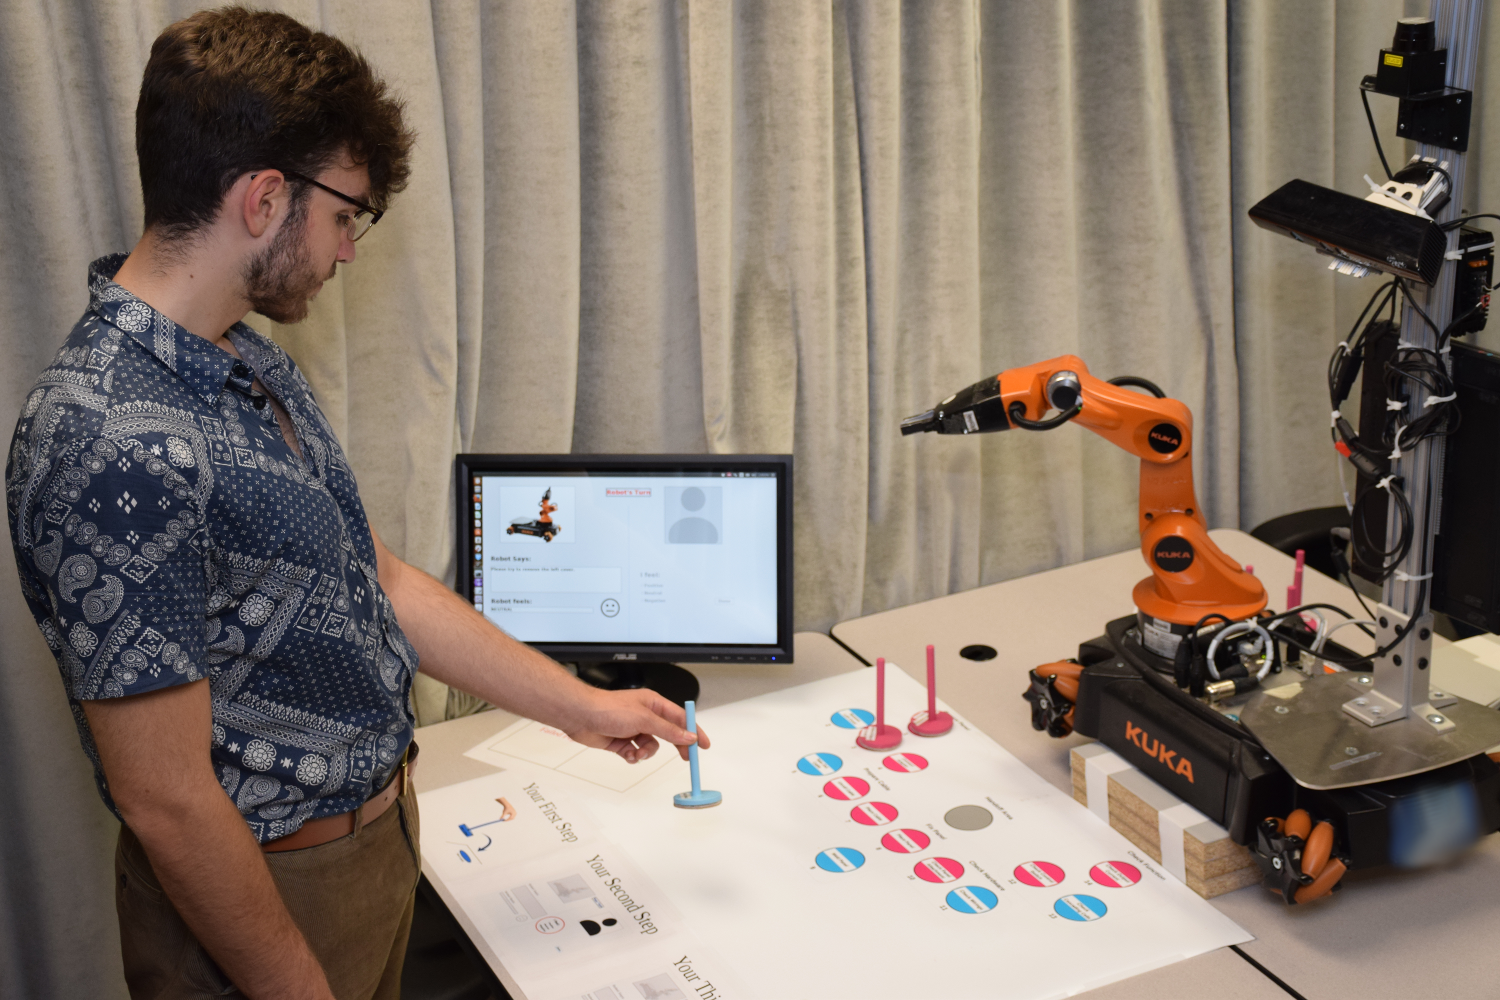
\includegraphics[scale=1.17]{figure/collaborative-robot.png}
    \caption{A robotic arm collaborating with a human to achieve a shared goal
    using \textit{Affective Motivational Collaboration Framework}.}
    \label{fig:collaborative-robot}
  \end{figure*}
  
  \item \textbf{Developing a computational framework based on \textit{Affective
  Motivational Collaboration Theory}:}

  (Chapter \ref{ch:framework}) In order to evaluate our computational models and
  algorithms within an interaction with human collaborators, we have developed
  a computational framework based on our theoretical foundations in
  \textit{Affective Motivational Collaboration Theory}. Our computational
  framework implements the key concepts related to \textit{Affective
  Motivational Collaboration Theory} as well as minimal implementation of other
  processes which are required for validation of the model but are not part of
  this thesis' contributions. The emphasis of the model is on the underlying
  cognitive processes of collaboration and appraisal concepts, rather than the
  Perception and the Action mechanisms.

  \item \textbf{Validating \textit{Affective Motivational Collaboration
  Theory:}}

  (Chapters \ref{ch:appraisals} and \ref{ch:awareness}) We have conducted two
  user studies a) to validate our appraisal algorithms before further
  development of our framework, and b) to investigate the overall functionality
  of our framework within an end-to-end system evaluation with human subjects
  and a robot. The second user study was also conducted to evaluate the benefit
  of using our computational framework in human-robot collaboration. In the
  first user study, we crowd sourced our questionnaires to test our hypothesis
  that humans and our algorithms will provide similar answers to questions
  related to different factors within our appraisal algorithms. In the second
  user study, we investigated the importance of emotional awareness in
  human-robot collaboration, and the overall functionality of the AMC framework
  with the participants in our study environment.
\end{enumerate}

\chapter{Background and Related Work}
\label{ch:background}

\section{Computational Collaboration Theories}

\subsection{Shared-Plans Theory}

\subsection{Joint-Intentions Theory}

\subsection{Hybrid Theories}

\subsection{Similarities and Differences}

\subsection{Applications of Collaboration Theories}

\section{Affective Computing}

\subsection{Affect and Emotions}

\subsection{Functions of Emotions}

\subsection{Motivation and Theory of Mind}

\section{Computational Models of Emotions}

\subsection{Appraisal Theory}

\subsection{Other Computational Models}

\subsection{Similarities and Differences}

\subsection{Applications in Autonomous Agents and Robots}

\chapter{Affective Motivational Collaboration Theory}
\label{ch:amct}

\section{Introduction}

\subsection{Scenario}

\subsection{Example of a Collaborative Interaction}

\section{Design and Architecture}

\subsection{Mechanisms}

\subsection{Functions of Emotions}

\subsection{Mental States}

\subsection{Attributes of Mental States}

\chapter{Appraisal Processes in Collaboration Context}
\label{ch:appraisals}

\section{Introduction}

\section{Appraisal and Collaboration}

\section{Appraisal Algorithms}

\subsection{Relevance}

\subsection{Desirability}

\subsection{Expectedness}

\subsection{Controllability}

\section{Methodology [This chapter will contain the crowdsourding study.]}

\section{Results and Evaluation}

\chapter{Computational Framework}
\label{ch:framework}

\section{System Overview}

\section{Components of the Architecture}

\subsection{Mental States}

\subsection{Collaboration}

\subsection{Appraisal}

\subsection{Coping}

\subsection{Motivation}

\subsection{Theory of Mind}

\subsection{Perception}

\subsection{Action}

\chapter{Improving Human-Robot Collaboration Using Emotional-Awareness}
\label{ch:awareness}

\section{Introduction}

As it was mentioned earlier, collaborative robots need to take into account
humans' internal states while making decisions during collaboration. Humans
express emotions to reveal their internal states in social contexts including
collaboration \cite{breazeal:sociable-interactive-robots}. Due to the existence
of such expressions robots' emotional-awareness can improve the quality of
collaboration in terms of humans' perception of performance and preferences.
Hence, collaborative robots need to include affect-driven mechanisms in their
decision making processes to be able to interpret and generate appropriate
responses and behaviors. Our aim in this setup was to study the importance of
emotional awareness and the underlying affect-driven processes in human-robot
collaboration. We examined how emotional-awareness impacts different aspects of
humans' preferences by comparing the results from our participants collaborating
with an emotion-aware and an emotion-ignorant robot.

\section{Collaborative Behaviors and Emotional-Awareness}

\subsection{Goal Postponement}

\subsection{Goal Management}

\subsection{Task Delegation}

\section{Implementation}
The implementation of this user-study included three separated parts. The first
part incorporated the Affective Motivational Collaboration Framework consisting
of all Mental Processes (see left-side of Figure \ref{fig:framework}) as we
described in Chapter \ref{ch:framework}. The second part was implemented to
receive action commands from the framework and forward them to the robot to
control joints and actuators (see right-side of Figure \ref{fig:framework}).
Finally, a wizard was the third part of this setting. The wizard did not do
anything but informing the robot/framework whether the current performed task by
either of the robot or the participant was achieved successfully. The act of the
wizard was completely invisible for the participants, and the wizard had not
impact on robot's decision other than providing tasks' failure or success.

\begin{figure*}[tbh]
  \centering
  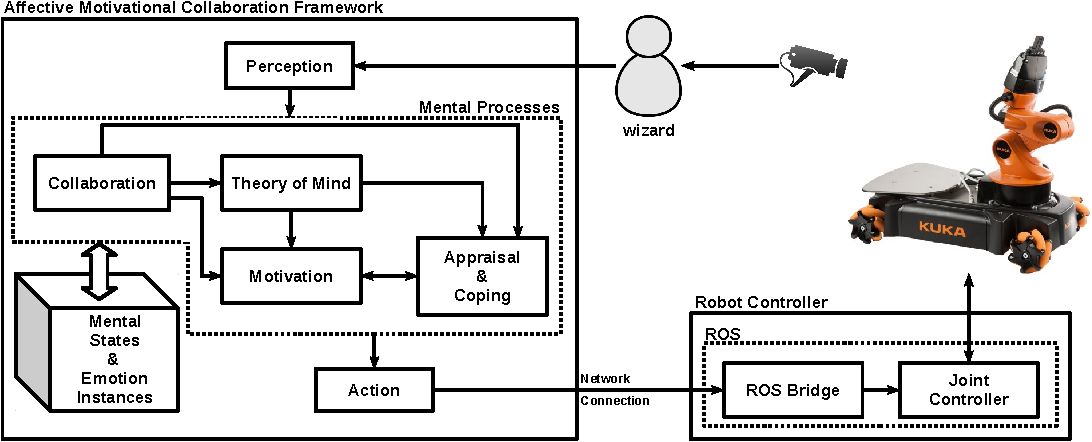
\includegraphics[width=\textwidth]{figure/framework-croped.pdf}
  \caption{{\fontsize{9}{9}\selectfont Computational framework based on
  [title suppressed for anonymity] theory (arrows indicate primary influences
  between mechanisms and data flow).}}
  \label{fig:framework}
  \vspace*{-5mm}
\end{figure*}

\subsection{Framework}
\label{sec:theory}
The framework includes all the mechanisms depicted as mental processes in Figure
\ref{fig:framework} along with the mental states. The mental
states shown in Figure \ref{fig:framework} comprise the knowledge base required
for all of the mechanisms in the overall model. The details about these mental
processes and mental states are described in Chapters \ref{ch:amct} and
\ref{ch:framework}. In this user-study, the Collaboration mechanism uses a
hierarchy of goals associated with tasks in a hierarchical task network
structure depicted in Figure \ref{fig:collaboration_structure}.

\begin{figure*}[tbh]
  \centering
  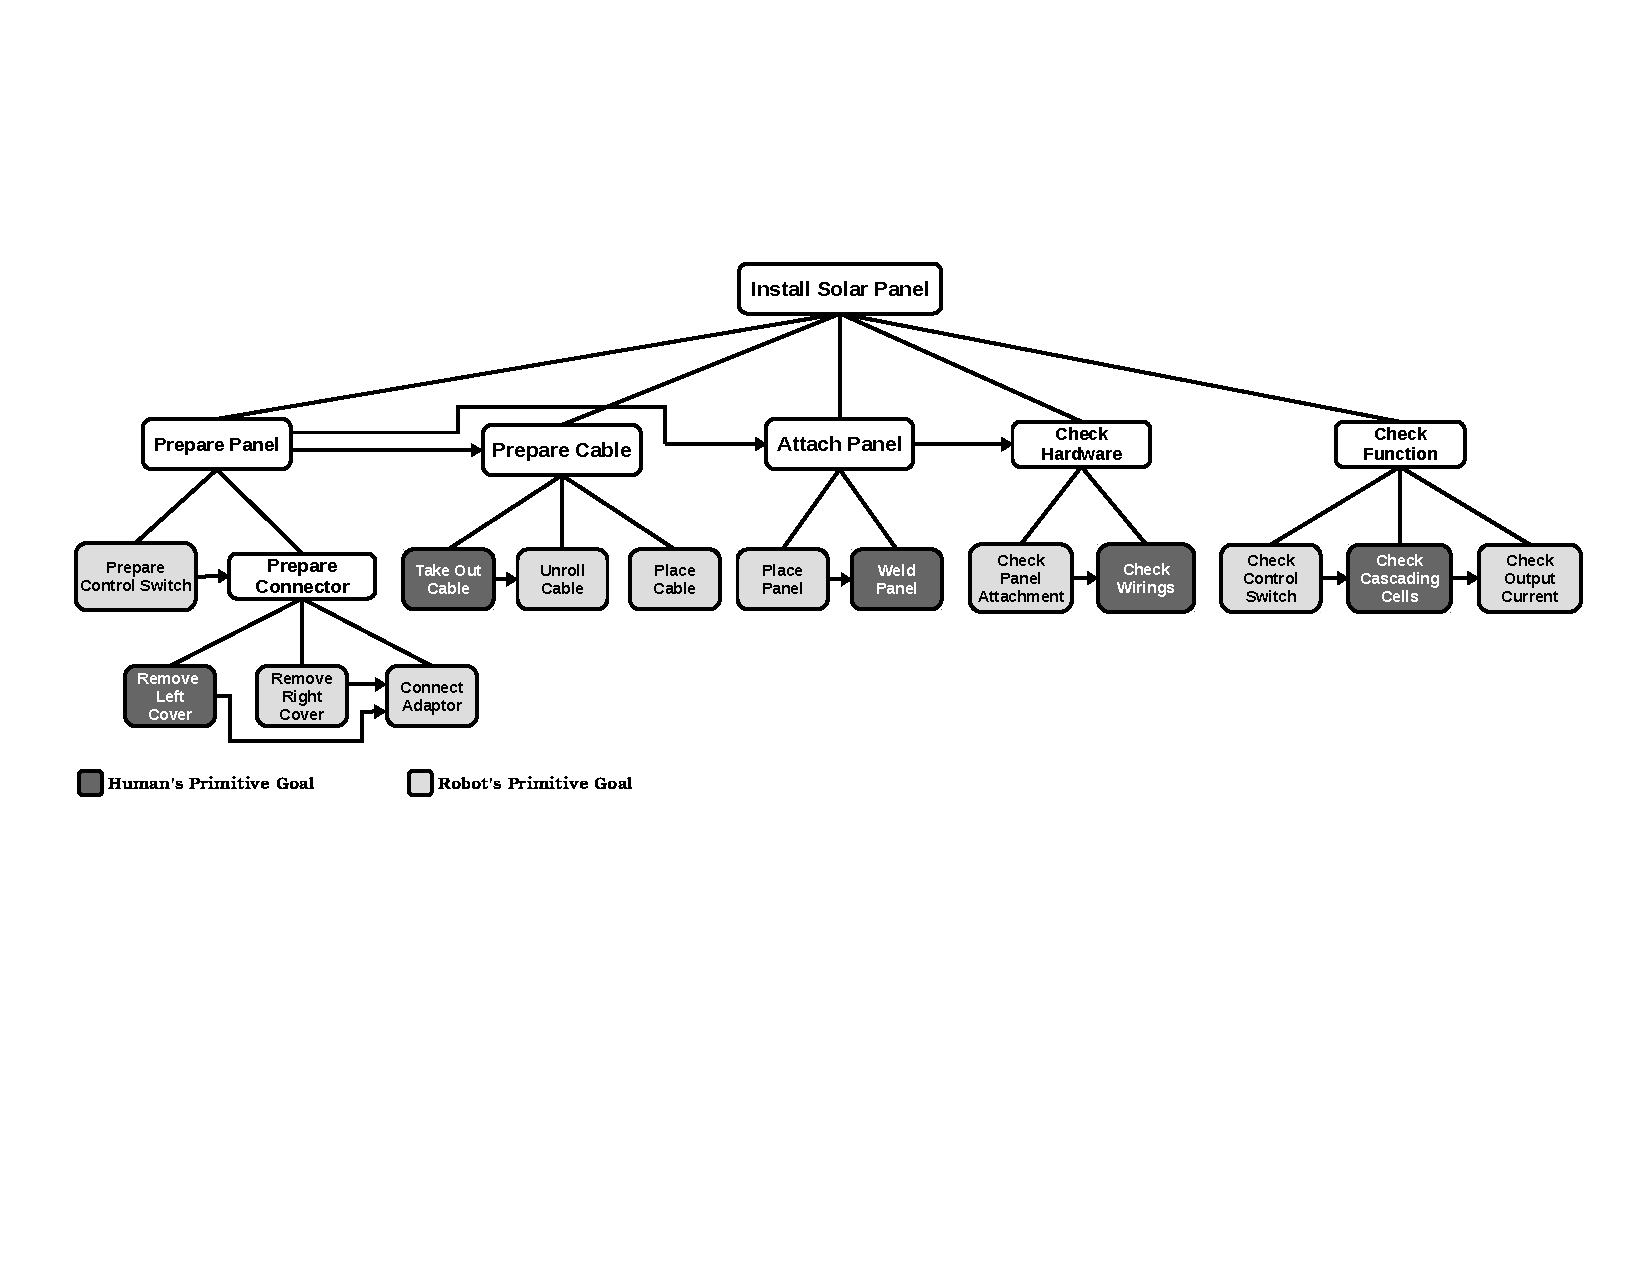
\includegraphics[width=1\textwidth]{figure/collaborationStructure.pdf}
  \caption{{\fontsize{9}{9}\selectfont Collaboration structure used as the
  task model.}}
  \label{fig:collaboration_structure}
  \vspace*{-5mm}
\end{figure*}

\subsection{Robot Controller}
The robot controller is comprised of two major components: 1) ROS-bridge and 2)
joint controller (see Figure \ref{fig:framework}).
ROS-bridge\footnote{http://wiki.ros.org/rosbridge\_suite} provides an API to ROS
functionality for non-ROS programs which enables us to send action commands from
our framework (implemented in JAVA) to the robot's joint controller. The joint
controller receives action commands and translates them into actual joint and
actuator commands and sends them to the robot.

\section{Experimental Scenario}

Our scenario was based on a table top turn-taking game that we designed to
simulate the installation of a solar panel. Participants had to collaborate
one-on-one with our robot to complete all the given tasks required to install
the solar panel. All the tasks consisted of picking up and placing
collaborators' available pegs on predefined spots on the board (see Figure
\ref{fig:game_board}). Each pick-and-place was associated with the robot's or
the participant's task. The robot and the participants had their own unique
primitive tasks that they had to accomplish in their own turn. The final goal of
installing a solar panel required the robot and the participants to accomplish
their own individual tasks. Failure of any task could create an impasse during
the collaboration.

\begin{figure}[tbh]
  \centering
  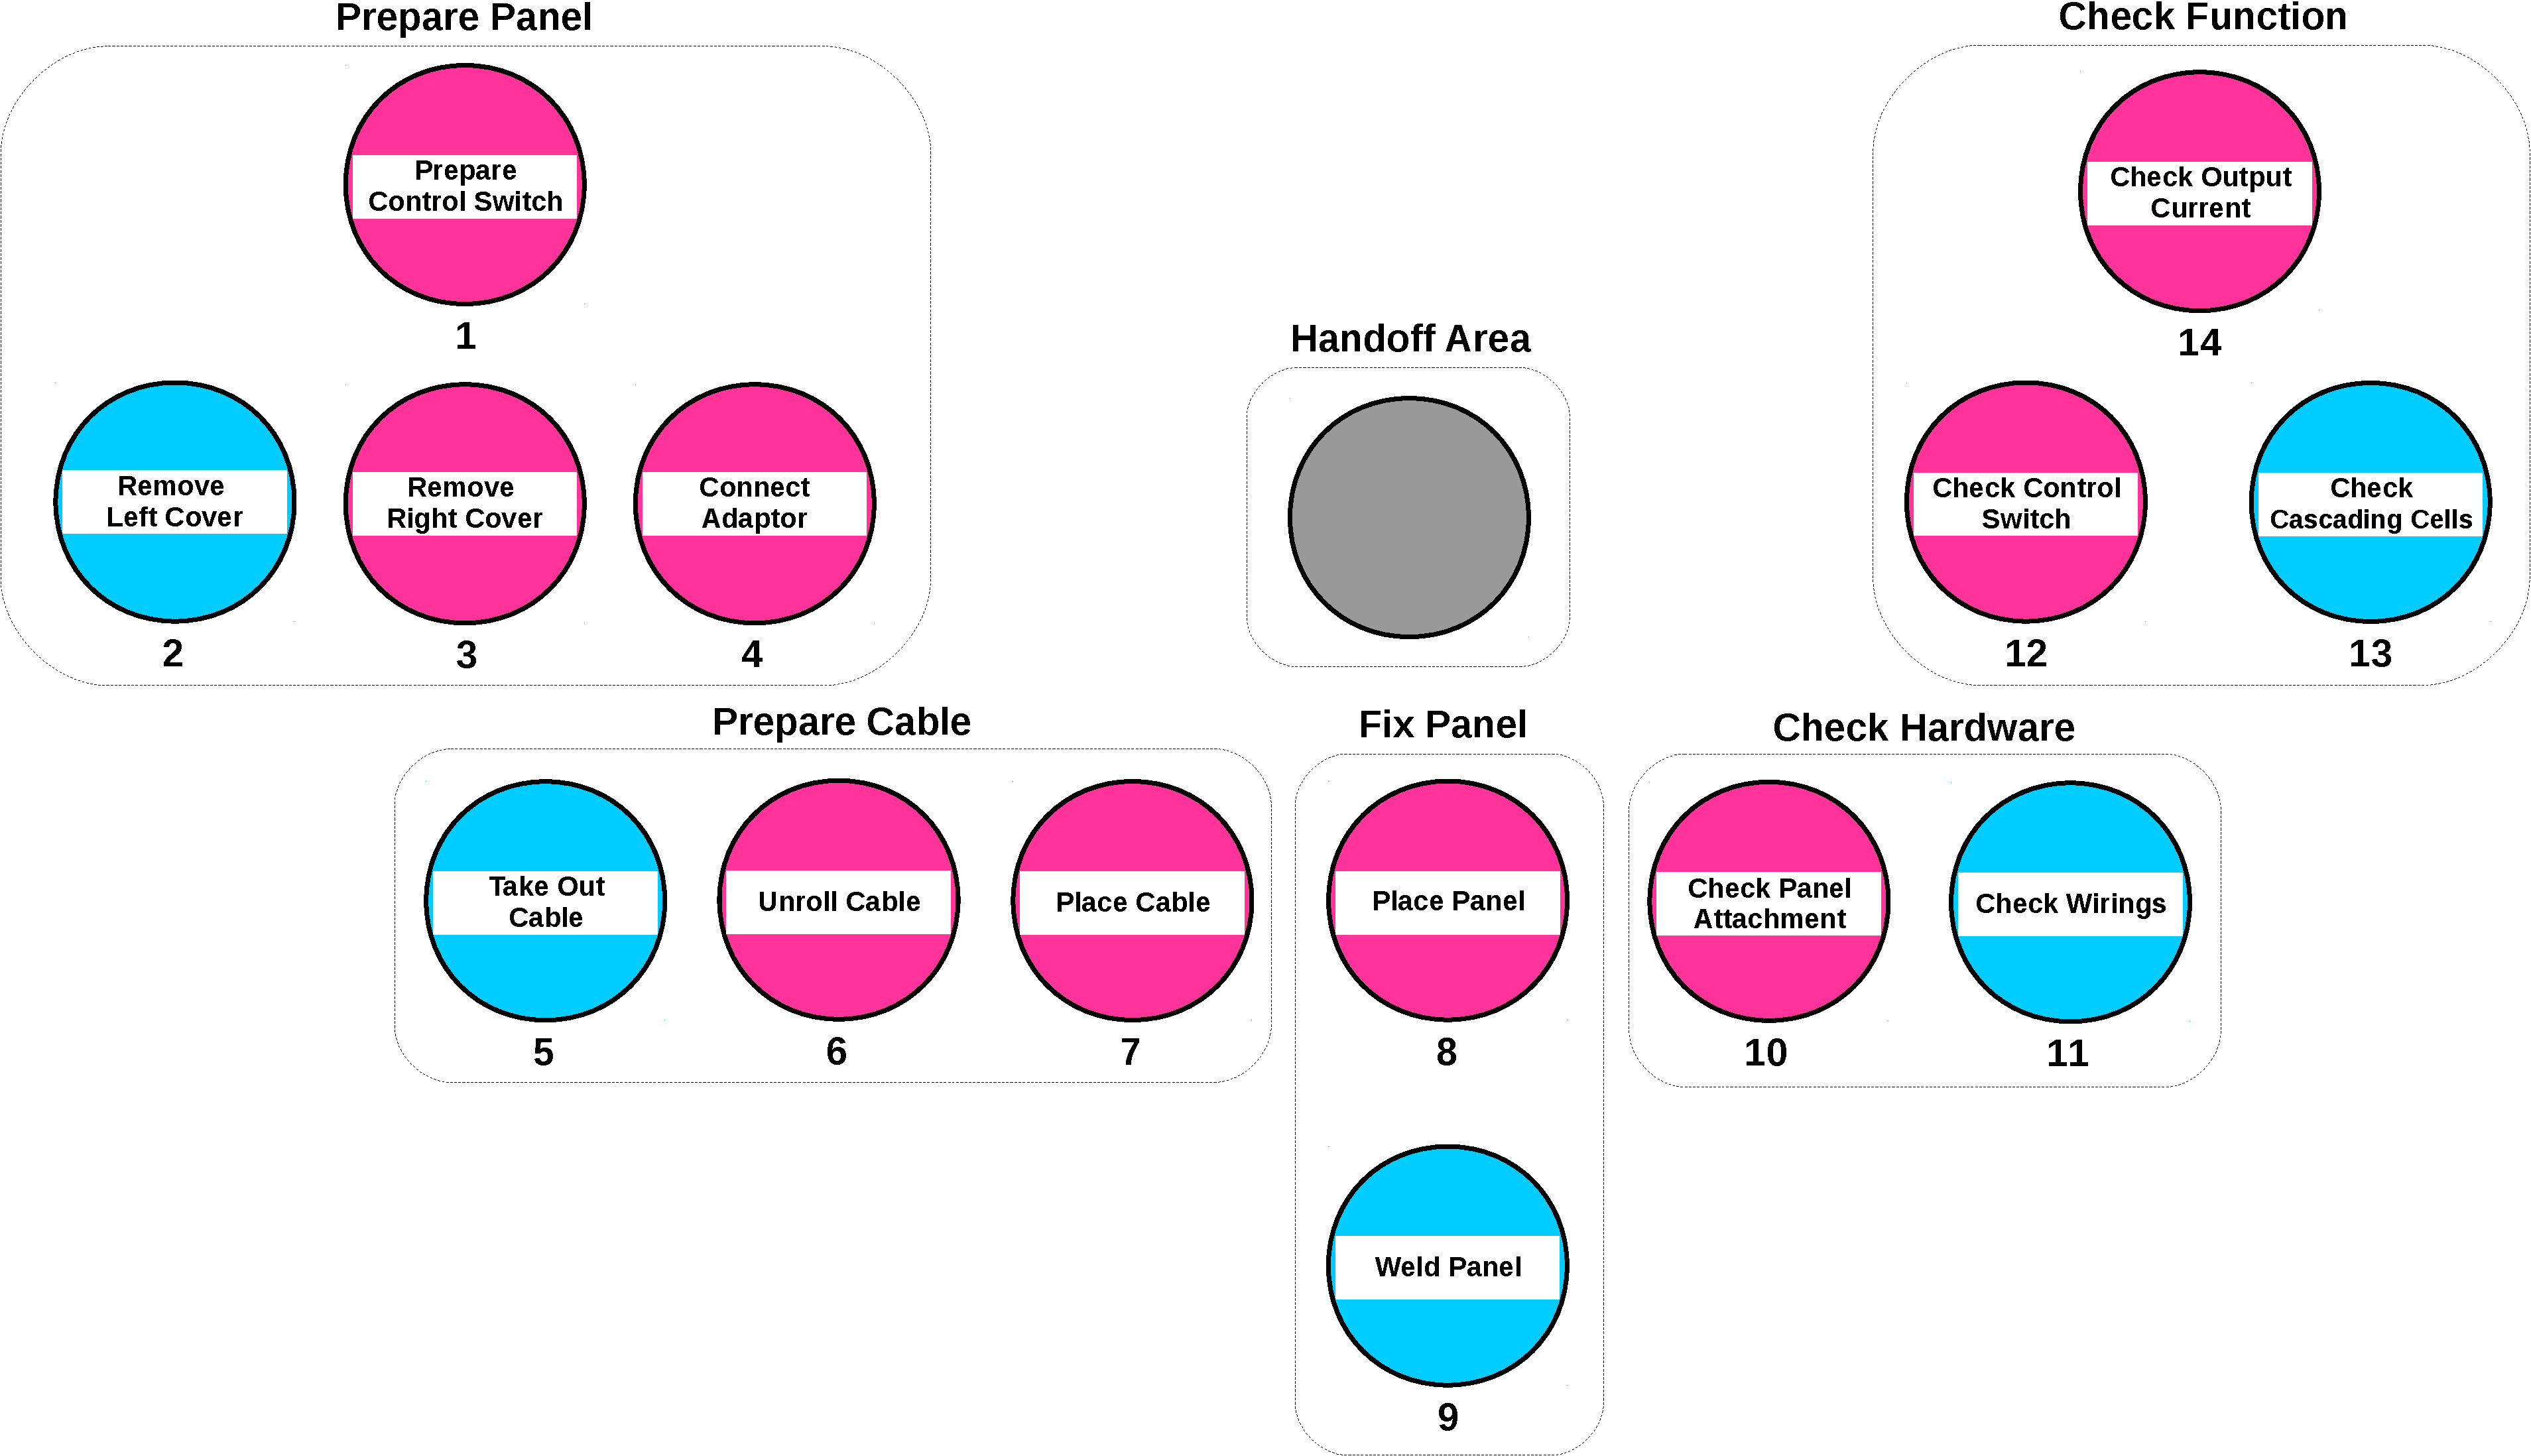
\includegraphics[width=1\textwidth]{figure/gameBoard.pdf}
  \caption{The layout of the available spots for the human and the robot to
  place their pegs during the collaboration.}
  \label{fig:game_board}
  \vspace*{-3mm}
\end{figure}

\subsection{The Robot}

We conducted our experiment based on a KUKA Youbot (see Figure
\ref{fig:environment}). The robot was stationary on top of a desk and was able
to pick up and place avaiable pegs corresponding to the robot's task. The robot
was operated based on Robot Operating System (ROS -- indigo) and was receiving
commands through the ROS-bridge from our [Title Suppressed For Anonymity]
framework (see Figure \ref{fig:framework}). We used a touch-screen monitor (see
Figure \ref{fig:environment}) to a) express robot's positive, negative or
neutral emotion through an emoticon, b) display robot's utterances, c)
control turn-taking process of the collaboration. and d) let the participants
express (report) their positive, negative or neutral emotion for each turn. The
robot used MaryTTS an open-source, multilingual Text-to-Speech Synthesis
platform to provide corresponding speech for its utterances in English.

\subsection{Interaction Paradigms}
\label{sec-interaction-paradigms}
At the beginning of each collaboration the robot asked each participant to
achieve the overall shared goal, i.e., ``installing the solar panel''. Then,
before working towards a new goal, the robot informed the participant about the
higher level nonprimitive goal (e.g. Prepare Panel -- see Figure
\ref{fig:taskModel}) of which the primitives were going to be working towards.
The same procedure was used by the robot if there was a decision to switch to
another nonprimitive due to the failure of a task in achieving the current goal.
After achieving a new primitive goal, the robot either informed the human that
it would pursue the next goal, or it informed and passed the turn to the human
to execute the next task with respect to the human's goal. In case of the
human's turn, the robot waited for the human to do a task, then the wizard let
the robot know whether the human's goal was achieved or not. Afterwards the
robot made a decision about which goal to pursue and informed the human
accordingly. The same procedure was applied to both conditions.

The robot interacted via a) speech, b) the corresponding utterance on the
screen, c) negative, positive and neutral expression of emotion through an
emoticon on the screen. There were two conditions of the robot: 1)
emotion-aware and 2) emotion ignorant. The robot used neutral expression in the
case of emotion-ignorance. The interaction was controlled autonomously by the
framework we discussed in Section \ref{sec:theory} in both the emotion-ignorant
and the emotion-aware cases. The reasoning about which task should be done and
controlling the robot was entirely autonomous. Only the perception of the task
failure or achievement by the robot or by the participant was done by a wizard
monitoring the collaboration outside of the test area. The interaction was
structured based on the exact same goals in an HTN for both conditions. The
robot was using the same utterances in both conditions. In the emotion-aware
condition the robot used a different behavior in comparison with the
emotion-ignorant condition only if the participant was expressing a negative
emotion in case of a failure; i.e., the robot's utterances were identical in
emotion-aware and emotion-ignorant cases if in the latter the participant
reported (expressed) a positive or a neutral emotion.

Three different behaviors could be generated only in the emotion-aware
condition. These three behaviors were 1) mitigating the human's negative emotion
and postponing its own task to help the human, 2) goal-management to switch to
another goal which has lower cost with respect to the human's negative emotion,
and 3) task delegation to the human to overcome the impasse. In each run, the
human had two pre-coordinated task failures, and the robot had one. If the human
expressed negative emotion after the first human task-failure, the robot
responded by mitigating the human's negative emotion by saying  ``It was not
your fault. I can help you with this task" and helping the human by providing a
peg to fulfill the human's task. If the human expressed negative emotion after
the second human task-failure, the robot informed the human that they could
proceed with another task to save time while simultaneously requesting a new peg
(i.e. help) from the supervisor. If the human expressed negative emotion as a
result of the robot's task failure, the robot requested help from the human (who
had the correct peg). In the event that the human expressed positive or neutral
emotion during these three failures, the robot behaved identically in the
emotion-ignorant and the emotion-aware cases, by asking the supervisor for help. 

\subsection{Environment and Tasks}

The environment was set up in the Human-Robot Interaction lab. and included the
robot, the collaboration board on top of a desk, and the participant standing in
front of the robot on the other side of the board (see Figure
\ref{fig:environment}). One of the experimenters monitored the interactions
using a live stream of a camera in a different room. The experimenter provided
only the required perception, i.e., decision on success or failure of the tasks
for the robot, through the entire time of the collaboration (see Section
\ref{sec-interaction-paradigms}).

The tasks were defined based on the HTN structure shown in Figure
\ref{fig:taskModel} and were executed in a turn-taking fashion by either of the
collaborators. For each task either the robot or the participant was responsible
to pick up one of the corresponding pegs from their own inventory and place it
on the right spot which was colored and tagged same as the associated peg. Some
pegs and corresponding spots on the board had hidden magnets which prevented the
pegs from standing upright. Any peg that fell over was considered a failed task. 

\section{Evaluation}
\subsection{Hypothesis}

The non/social functions of emotions impact a collaboration process. Human
collaborators prefer to collaborate with others whose behaviors are influenced
by these functions of emotions depending on the context. We developed seven
hypotheses on positive influence of emotion-awareness and usefulness of emotion
function during collaboration:

\textit{\textbf{Hypothesis 1.}} Subjects will feel closer (likability) to the
emotion-aware robot rather than the emotion-ignorant robot.

\textit{\textbf{Hypothesis 2.}} Subjects will find the emotion-aware robot to be
more trustworthy than the emotion-ignorant robot.

\textit{\textbf{Hypothesis 3.}} Subjects will find the emotion-aware robot to
have better performance in collaboration than the emotion-ignorant robot.

\textit{\textbf{Hypothesis 4.}} Subjects will find the emotion-aware robot to be
more understanding of their feelings than the emotion-ignorant robot.

\textit{\textbf{Hypothesis 5.}} Subjects will find the emotion-aware robot to be
more understanding of their goals than the emotion-ignorant robot.

\textit{\textbf{Hypothesis 6.}} Subjects will feel more satisfied about the
collaboration when working with the emotion-aware robot rather than
emotion-ignorant robot.

\textit{\textbf{Hypothesis 7.}} Subjects will perceive higher level of mutual
satisfaction with emotion-aware robot than emotion-ignorant robot.

\begin{figure}
  \centering
  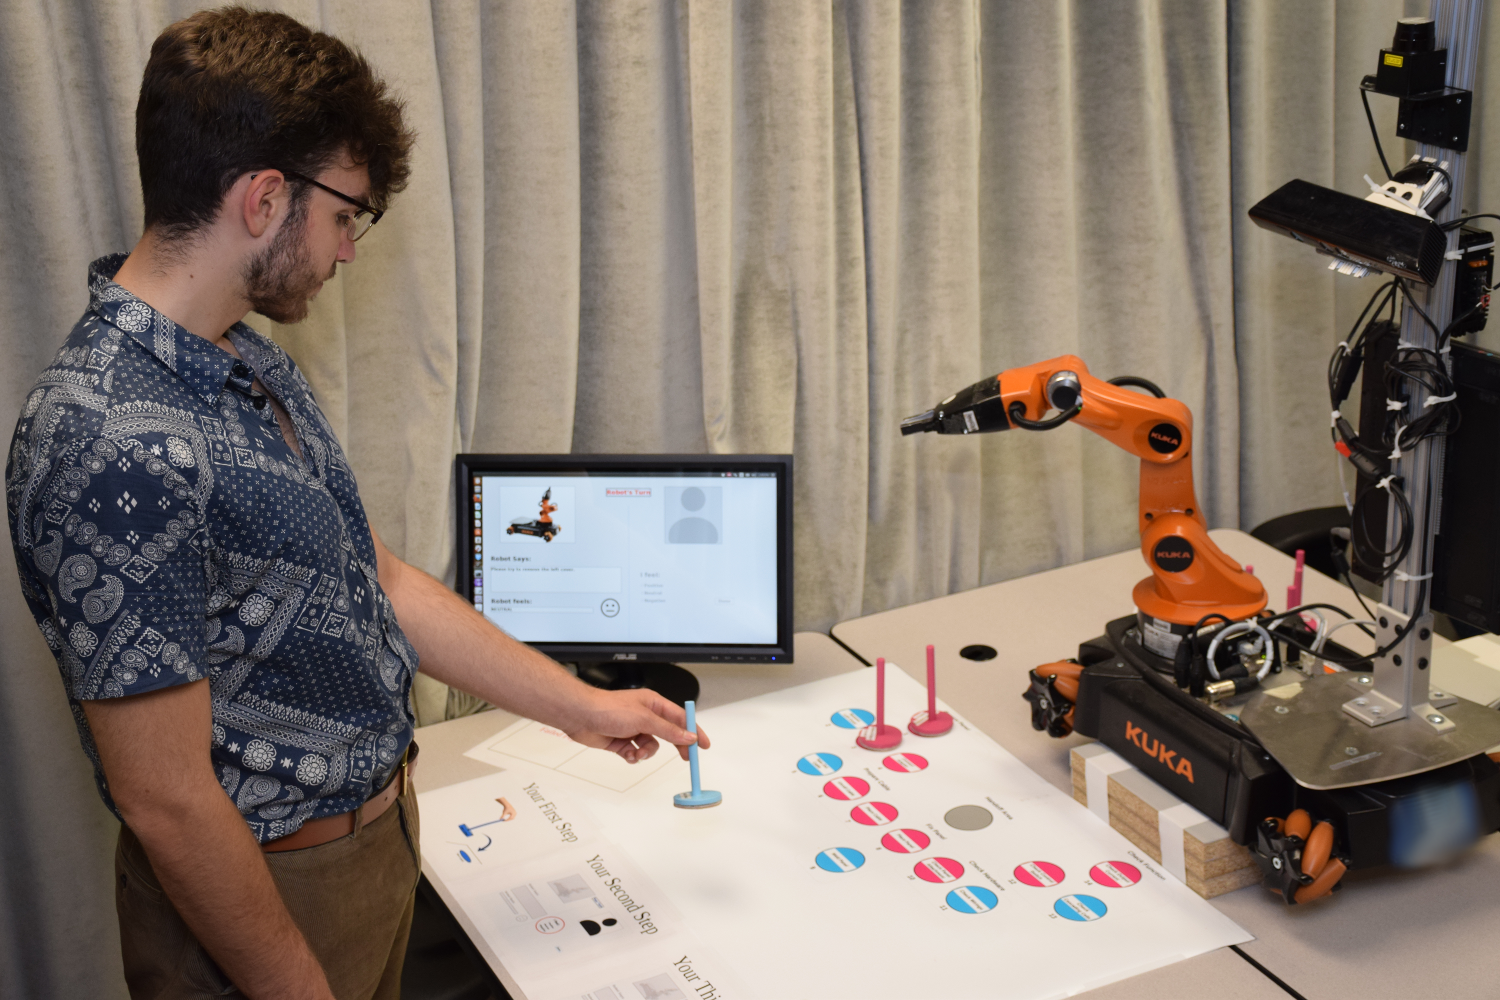
\includegraphics[width=1\textwidth]{figure/environment.png}
  \caption{{\fontsize{9}{9}\selectfont Experimental setup.}}
  \label{fig:environment}
  \vspace*{-5mm}
\end{figure}

\vspace*{3mm}
\subsection{Procedure}
\label{sec:procedure}
Participants were first given a brief description of the purpose of the
experiment. After the short introduction, they were asked to review and sign a
consent form. Participants were then provided with a written instruction of
their task and the rules for collaborating with the robot. Then, one of the
experimenters lead them into the experiment room and asked the participants
to asked to answer pre-experiment questionnaires. Afterwards, the experimenter
went through all the details of the instructions with the participants
standing in front of the collaboration board and the robot. The experimenter
confirmed participants' correct understanding of the tasks and informed them
of types of task failures that might occur during the collaboration.
Participants were told that researchers were developing a collaborative robot
and would like their help in evaluating their design. Participants were provided
with identical instructions and randomly assigned to the conditions in the
experiment. They were told that, after their collaboration with the robot, they
would be asked to answer a questionnaire on their experience. After completing
the first round of collaboration, participants answered a post-experiment
questionnaire that measured their perceptions of the robot, the task, and
the collaboration procedure. After answering the first post-experiment
questionnaire, participants were told that they were going to collaborate with
the robot one more time and the robot might not necessarily have the same
collaborative behavior. After completing the second round of collaboration,
participants were asked to answer the second post-experiment questionnaire which
consisted of the same questions as the first post-experiment questionnaire.
After all, participants were asked to answer an open-ended questionnaire which
measured their perception of difference between two runs, their preference of
collaborative robot between two runs, and their reasons of preference.

\subsection{Measurements}
\label{sec:Measurements}
In our study two basic conditions of the robot were tested: a) the
emotion-ignorant condition, b) the emotion-aware condition. We measured
participants' recall of the collaborative behaviors presented by the robot using
an open-ended post-experiment questionnaire. We also specifically asked the
participants what behavior of the robot they liked during their collaboration.
We also evaluated participants' levels of satisfaction, trust, confusion, goal
achievement, mutual understanding of goals, mutual understanding of feelings,
mutual agreement, and also participants' beliefs about the efficiency of
collaboration and their feeling of robot's collaborative behaviors. Seven-point
Likert scales were used in these questionnaire items.

\subsection{Participants}
\label{sec:Participants}
A total of 37 participants participated in the experiment in 74 trials.
Participants were recruited from Worcester Polytechnic Institute's students and
staffs as well as other civilians recruited from outside of the campus. The ages
of the participants varied between 19 and 74 with an average of 34.2 years
before our screening of 4 subjects based on our sanity check questions. After
this screening the ages of the participants varied between 19 and 54 with an
average of 30.8 years old. Of the 33 participants, 21 were female and 12
were male. Each participant participated in 2 trials. In one trial the robot was
aware of human's emotion and in the second trial the robot was ignoring human's
emotion. The order of these two trials were randomly assigned to each
participant. In general we used emotion-ignorant robot first in 16 experiments,
and emotion-aware robot first in 17 experiments.

\begin{sidewaysfigure}
\centering
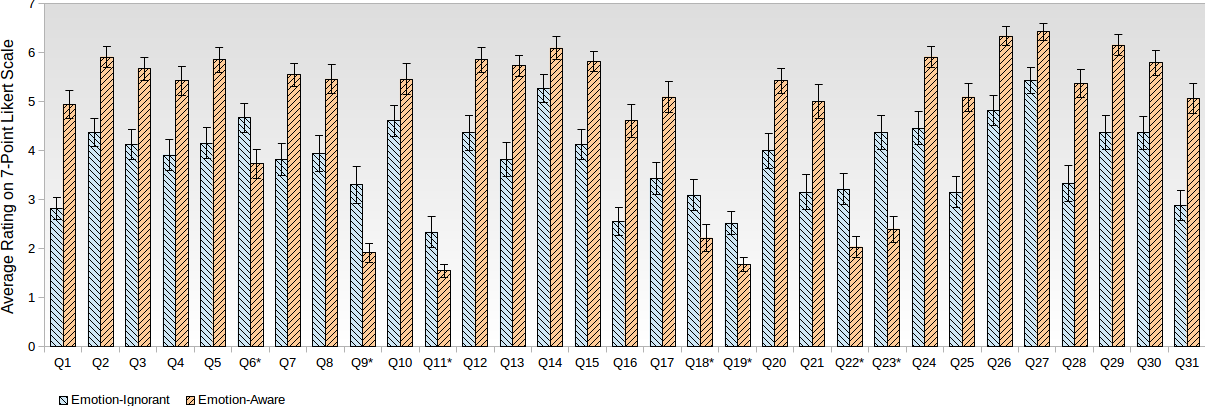
\includegraphics[width=1\textwidth]{figure/31questions.png}
\caption{Results of the Likert scale surveys for 31 questions. The p-value for
the difference between the means for each question is <0.001, except for Q????,
which is 0.008.}
\label{fig:14Questions}
\end{sidewaysfigure}

\begin{figure*}[tbh]
\centering
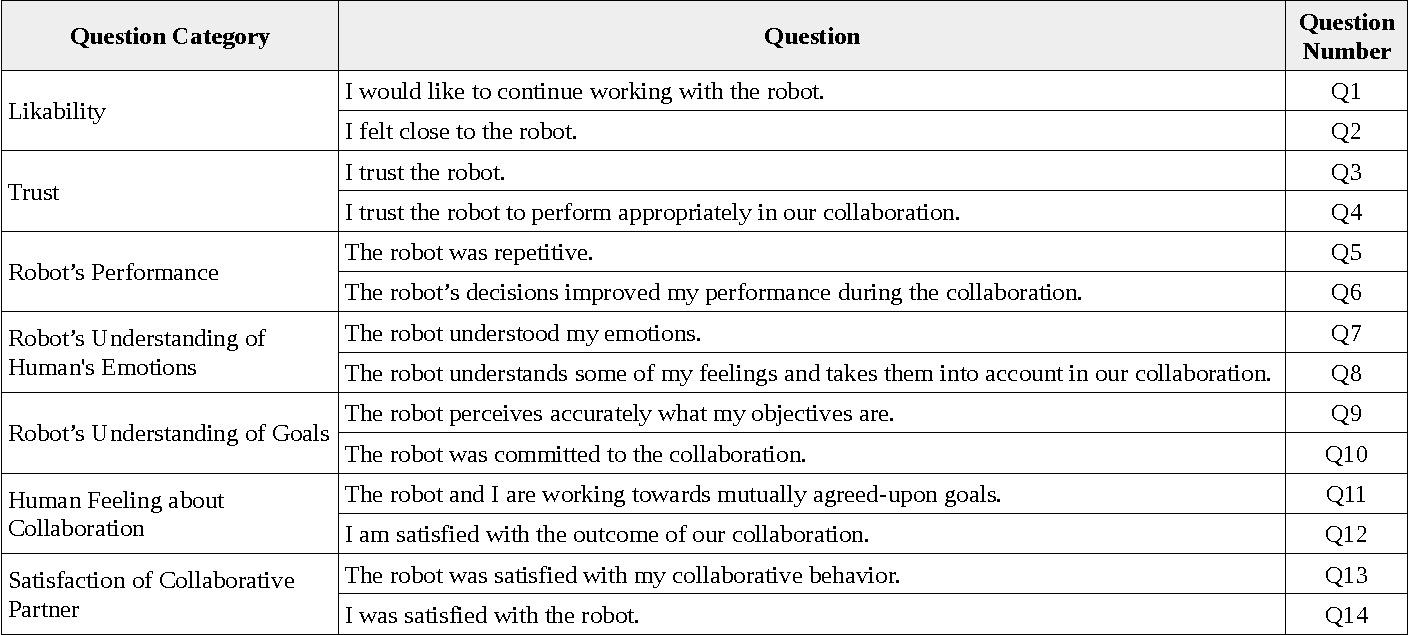
\includegraphics[width=1\textwidth]{figure/table1-croped.pdf}
\caption{The 14 Likert scale questions presented in this paper, organized
according to their groups.}
\label{fig:14Questions-Table}
\end{figure*}

\begin{figure*}[tbh]
\centering
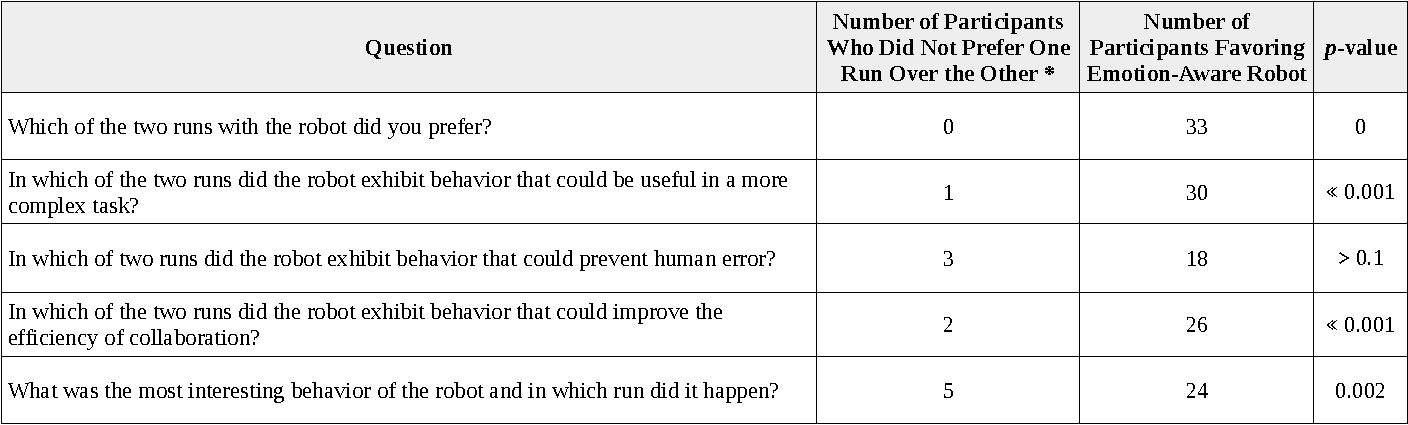
\includegraphics[width=1\textwidth]{figure/table2-croped.pdf}
\caption{Open-ended questionnaire questions and results.}
\label{fig:Open-Ended-Table}
\label{fig:14Questions}
\vspace*{-5mm}
\end{figure*}

\begin{figure*}[tbh]
\centering
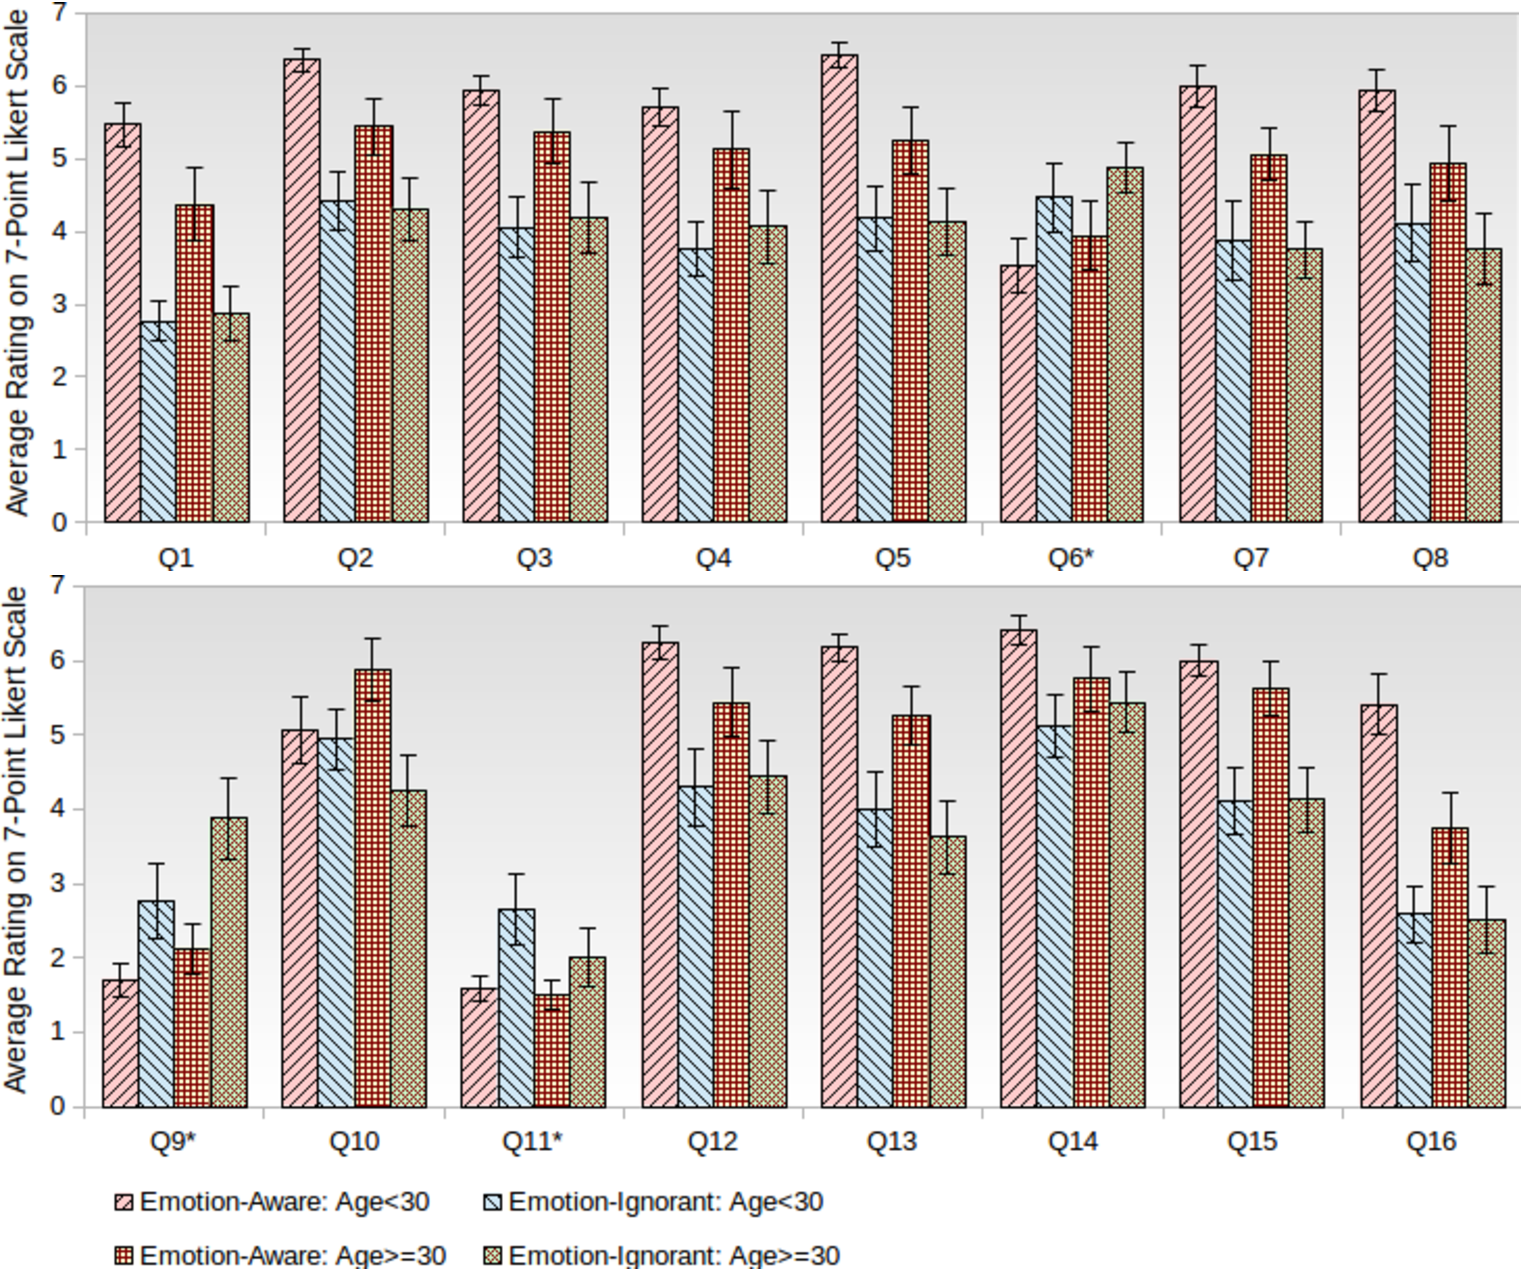
\includegraphics[width=1\textwidth]{figure/AgeComparison1_2.pdf}
\caption{Impact of age on results of Likert scale Questions 1-16}
\end{figure*}

\vspace*{-3mm}
\section{Results}

As discussed in Section \ref{sec:Measurements}, results of the user study were
gathered through a 31-question Likert-scale survey that was given to each participant
after each run with the robot, and through a 5-question open-ended summary
questionnaire at the end of the experiment.

\subsection{7-Point Likert Scale Survey Results}
As mentioned previously, the 7-point Likert scale survey was administered at
the end of the emotion-ignorant run and at the end of the emotion-aware run for
each participant. The 31 questions are generally categorized to evaluate the
humans' perceptions of the following seven categories, with 3-6 questions per
group: (1) the likability of the robot (2) the level of trust the human feels
in the robot (3) the human's perception of the robot's performance (4) the
human's perception of the robot's understanding of human's emotions (5) the
human's perception of the robot's understanding of human's and collaboration's
goals and objectives (6) the human's feeling about the collaboration and (7)
the human's perception of the human's and robot's mutual satisfaction with each
other as collaborative partners. Of the 31 questions, 2 were chosen from each
group, for a total of 14 questions, for presentation in this paper. The
remaining questions were omitted due to space constraints. The questions
presented are provided in Figure \ref{fig:14Questions-Table}. These questions
are chosen as representative of their respective groups of questions, and their
results do not necessarily represent the highest levels of statistical
significance.

\begin{figure*}[tbh]
\centering
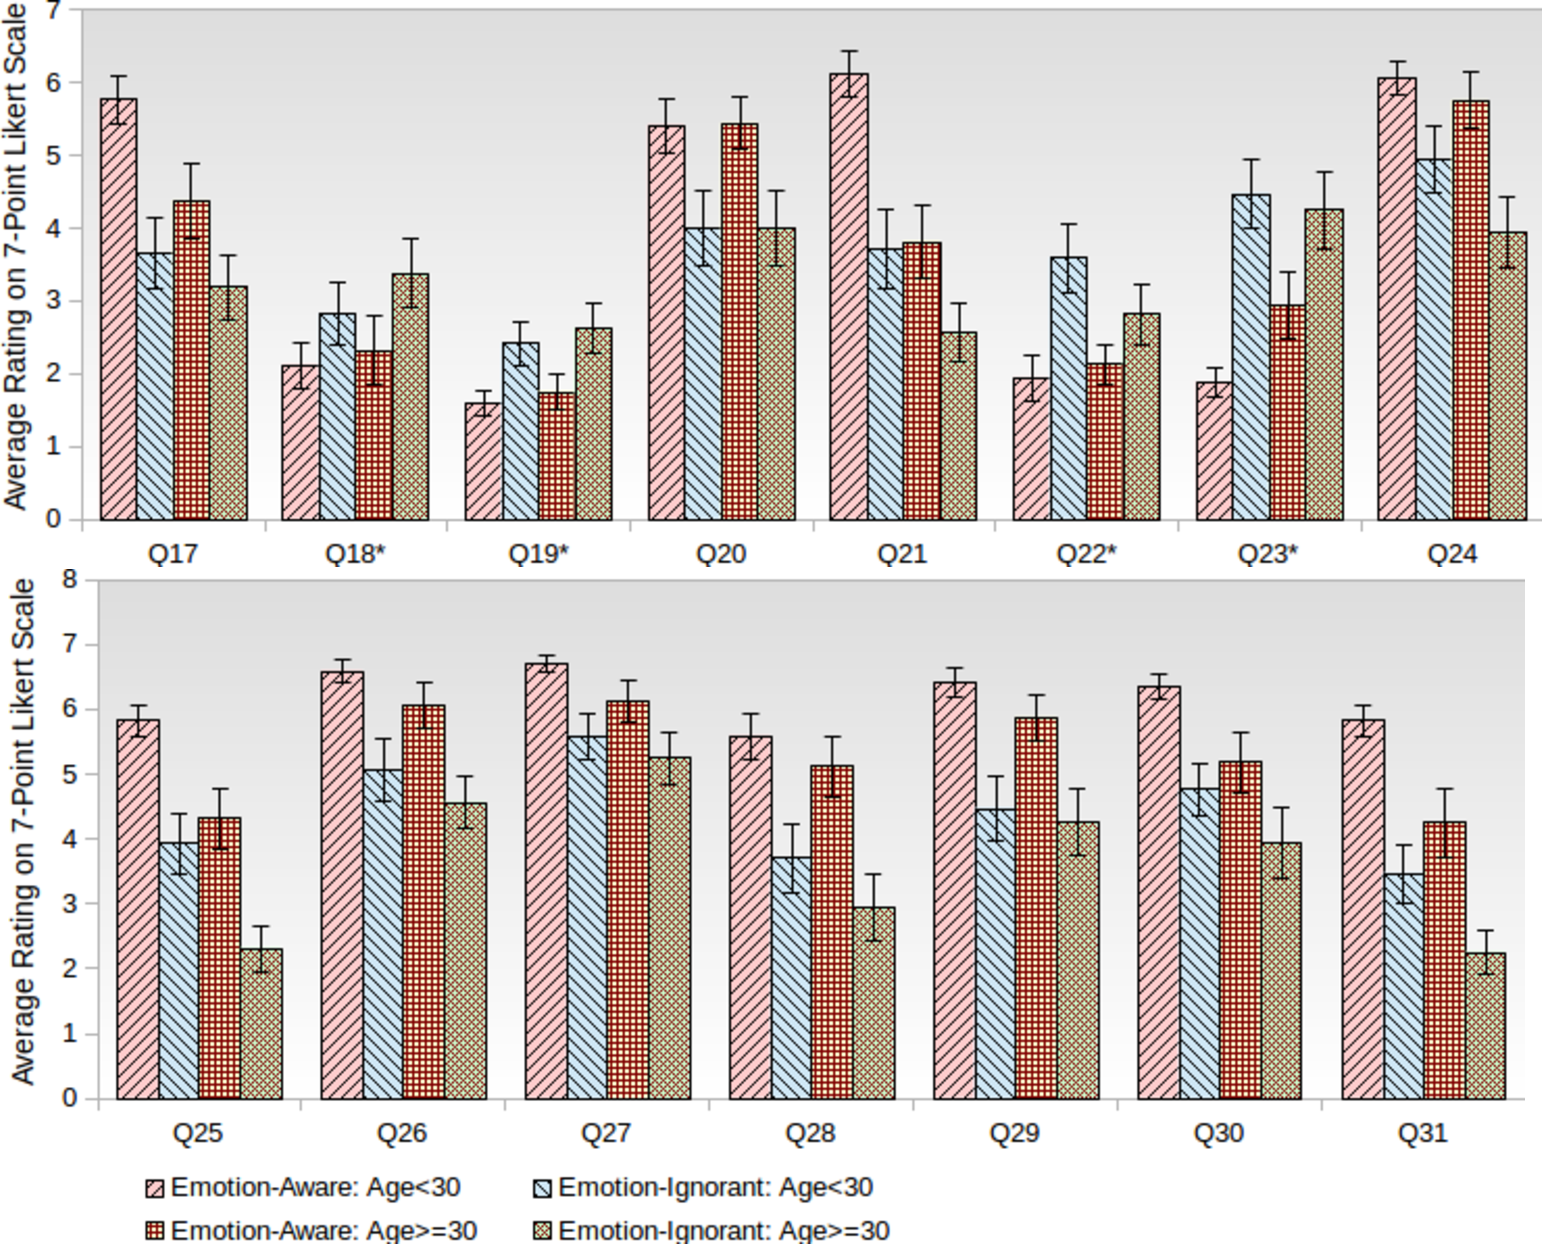
\includegraphics[width=1\textwidth]{figure/AgeComparison3_4.pdf}
\caption{Impact of age on results of Likert scale Questions 17-31}
\end{figure*}

The results were analyzed using a two-tailed paired t-test to analyze the
difference of means between the emotion ignorant and the emotion-aware
condition. Refer to Figure \ref{fig:14Questions} for the results. As mentioned
in Section \ref{sec:Participants}, participants were randomly assigned to complete
either the emotion-ignorant or the emotion-aware run first; analysis of the
results revealed no statistically significant difference or consistent pattern
based on which run the participant completed first.

\subsubsection{Likability of the Robot}
\label{sec:Likability}
Questions 1 and 2 addressed the likability of the robot. As shown in Figure
\ref{fig:14Questions}, participants would like to continue working with the emotion-aware
robot significantly more than the emotion-ignorant robot by an average of about 1.5
points; additionally participants felt more close to the emotion-aware robot
than the emotion-ignorant robot by about 2.1 points, on the 7-point scale. This
supports Hypothesis 1, which stated that humans would prefer to work with the
emotion-aware robot over the emotion-ignorant robot.

\subsubsection{Human Trust in the Robot}
\label{sec:Trust}
Questions 3 and 4 were designed to measure the degree of trust that the human
participants felt in the robot. As shown in Figure \ref{fig:14Questions},
participants trusted the emotion-aware robot an average of 1.5 points more than
the emotion-ignorant robot, both in general and in terms of collaboration
performance. In fact, in Question 4, participants rated their trust in the
emotion-aware robot to perform appropriately during collaboration an average of
5.9 on a 7-point Likert scale, where 7.0 would indicate maximum trust; this
indicates that the participants felt that the emotion-aware robot's
collaborative performance was acceptable. This result supports Hypothesis 2,
that posits that human participants would find the emotion-aware robot to be
more trustworthy than the emotion-ignorant robot.

\subsubsection{Perception of the Robot's Performance} 
\label{sec:Performance}
Question 5 (which is reverse-scored) measures the participant's perception of
repetitiveness in the robot during the collaboration. In both conditions,
participants rated the robot as moderately repetitive, with the emotion-ignorant
robot's average response being about 1.1 points higher than the emotion-aware.
This result correlates with several of the open-ended responses which described
the emotion-aware robot's behaviors as ``cute'' and ``interesting'', refer to
Section \ref{sec:Open-Ended}. The participants also felt that the emotion-aware
robot's decisions during collaboration improved their own performance, with an
average rating of 5.4, while the emotion-ignorant robot only received an average
rating of 3.3, indicating that participants felt it was not able to interact in
such a way as to increase the human's performance; refer to results from
Question 6. These results support Hypothesis 3, which posited that humans will
perceive the emotion-aware robot as being more capable than the emotion-ignorant
robot.

\subsubsection{Robot's Understanding of Human Emotions} 
\label{sec:Emotions}
For Questions 7 and 8, participants ranked the emotion-aware robot's
understanding of emotions 2.2 and 1.8 points higher, respectively, than the
emotion-ignorant robot's understanding of emotions, supporting Hypothesis 4.
This category showed the highest total difference between the emotion-ignorant
and the emotion-aware robot.

\subsubsection{Robot's Understanding of Human and Collaboration Goals}
\label{sec:Goals}
Question 9 was a measure of whether the human perceived that the robot cared
about the human's goal. On average, participants provided an average rating for
the emotion-aware robot that was 1.5 points higher than that for the
emotion-ignorant robot. Question 10 measured the human perception of the
robot's commitment to the collaboration; for this measure, the average
participant score assigned to the emotion-aware robot was 6.2 points out of a
maximum of 7 points, indicating that the participants felt that the
emotion-aware robot was strongly committed to the collaboration. The
emotion-ignorant robot received an average rating of 4.4 points, indicating
only moderate commitment. These results strongly support Hypothesis 5, which
posits that humans will feel that the emotion-aware robot will better understand
their goals than the emotion-ignorant robot.

\subsubsection{Human's Feeling about the Collaboration}
\label{sec:Collaboration}
Questions 11 and 12 were designed to gauge how the human participants felt
about the partnership within the collaboration and the outcome of the
collaboration. In the emotion-aware condition, participants scored Questions 11
and 12 as 6.1 and 6.3, respectively, indicating a strong sense of pursuing
mutually agreed-upon goals and very high satisfaction with the overall
collaboration. It is worth noting that the participants scored Question 11 for
the emotion-ignorant case at 5.3 points, leading to a 0.8-point difference
between the two conditions; this is the smallest gap that occurs between the
results for any question, and indicates that the participants felt that the
goals were still partially mutually agreed-upon in the emotion-ignorant case.
However, the general satisfaction with the outcome of the collaboration was
significantly less in the case of the emotion-ignorant robot, at 4.8 points.
These results support Hypothesis 6 that humans will feel greater a greater sense
of mutual collaboration and understanding about the collaboration with the
emotion-aware robot.

\subsubsection{Human Perception of Mutual Satisfaction with Collaborative
Partner}
\label{sec:MutualSatisfaction}
Questions 13 and 14 were designed to measure the human's perception of the
robot's satisfaction with the human, and the human's satisfaction with the
robot, respectively. The participants provided an average response in the
emotion-aware condition of 5.8 and 5.9 to Questions 13 and 14, respectively,
indicating a high level of mutual satisfaction; both answers were about 1.5
lower, on average, in the emotion-ignorant condition. These results indicate a
higher level of satisfaction working with the robot in the emotion-aware
condition, and strongly support Hypothesis 7, which posited that humans will
feel a greater sense of mutual satisfaction with the emotion-aware robot than
the emotion-ignorant robot.

\subsection{Results from the Open-Ended Questionnaire} 
\label{sec:Open-Ended}
As described in Section \ref{sec:procedure}, each participant answered an open-ended
questionnaire at the end of the study. Figure \ref{fig:Open-Ended-Table}
summarizes the questionnaire and which run users preferred for certain
conditions (i.e. emotion-ignorant or emotion-aware). Note that some users either
chose not to state a preference, or provided ambiguous answers regarding which
run they preferred for certain conditions; these results were removed from the analysis.
As shown in Figure \ref{fig:Open-Ended-Table}, 100\% of users unambiguously
preferred the run with the emotion-aware robot. In general, this preference
stemmed from a feeling of closeness and partnership, as seen in these responses:
``the robot had emotions and responded to my emotions. Also, what it said about
my failing was cute and aimed to make me feel better.'' Another example is ``I
liked feeling needed and accounted for; I felt closer to the robot.'' Finally,
``I saw the changes in its feeling, which motivated me to care more about my
act...I also liked that he asked me to correct its failure, although it could
ask the supervisor.''  

When asked in which of the two runs the robot exhibited
behavior that could be useful in a more complex task, 93.75\% chose the
emotion-aware robot. In general, respondents thought that the emotion-aware
robot was better at problem solving, more adaptable, and more capable of
handling the social complexities that occur in collaboration, as shown in
responses such as ``The robot explained motives...which is important to keep a
team communicating and on the same pace.'' Also, ``When we failed he initially
switched to a new task and then came back to the originally failed task. It kept
me from getting irritated and negative.'' Finally, ``The more complex, the more
necessary it is to understand how humans think and operate...an empathetic robot
can adapt, encourage and help.'' It is worth noting that one respondent
preferred the emotion-ignorant case, saying ``In a more complex task it might be
better for the robot to take control and simply tell me what to do; trying to be
understanding and collaborative wouldn't be as important as doing the task
correctly.''

The only question that did not provide statistically significant support in
favor of the emotion-aware robot related to which case the robot exhibited
behavior that could prevent human error. About 40\% of respondents thought that
the emotion-ignorant robot was more likely to prevent human error; however, all
but one of these cited calling the supervisor as the main method of preventing
human error, in spite of the fact that the instructions indicated that the
robot's need to call the supervisor counted against the collaboration. Of the
60\% who thought that the emotion-aware robot was better at preventing human
error, most cited the robot's ability to console the human as the main behavior
that could prevent human error. Respondents indicated that this enabled them to
move on and feel better about the collaboration, as with this response: ``The
robot switched to a different task and we came back to an error later. This
allowed my mind to move away from being frustrated. I was able to complete a
different task which felt like a win - then come back and finish the error.
Making my mind move away from frustration could definitely prevent more
errors.''

When asked in which of the runs the robot exhibited behavior that could improve
the efficiency of the collaboration, 83.9\% responded with the emotion-aware
case; of these, the vast majority stated that this was because of the robot's
ability to change the order of tasks in the event of a failure, and to ask the
human for help.

Finally, when asked in which run the most interesting behavior occurred, 82.8\%
chose the emotion-aware condition. Of these respondents, 12 individuals stated
that the robot's attempt to console the human by saying ``It was not your
fault'' in response to the human's negative emotion that occurred as a
consequence of the human's failed task was the most interesting behavior, and a
majority mentioned that it actually made them feel more positive. Six
participants referred to the robot's ability to understand and express emotion.
Several participants referred to the robot's ability to communicate, including
the ability to ask questions. Of those who responded with the emotion-ignorant
case, most found the ability to call the supervisor, and mechanical functions,
such as gripping, to be most interesting.

\subsection{Impact of Demographics} 
As mentioned in Section \ref{sec:Participants}, we recorded certain demographic
information from each participant, including age and gender. We also had each
participant complete several personality questionnaires. Although it was not the
primary purpose of the study, we investigated the Likert scale results to
determine if there were any relevant trends based on the demographics and
personalities of the participants. A close study of the results did  not reveal
any identifiable pattern based on gender or personality.

Age did reveal an interesting pattern. We divided the participants into two
groups, below 30 years of age and 30 or above. While question-by-question
comparisons revealed only a few statistically significant differences based on
age, a consistent pattern emerged. For each of the fourteen questions presented,
the younger age group reported higher scores for the emotion-aware robot (except
Question 5, which is a reverse-score question). In the emotion-ignorant case,
the younger group still scores the robot higher than the older group for 9
questions; for the other 5 questions, the older group scores the
emotion-ignorant robot higher. In fact, a pattern emerged in which the score
drop between the emotion-aware and the emotion-ignorant case was more for the
younger group than for the older group; only questions 4, 6 and 12 broke this
pattern.

\vspace*{-2mm}
\section{Discussion}
Based on the results, all participants prefer to work with the emotion-aware
robot. Humans find the emotion-aware robot more likable and more trustworthy, as
indicated in the Likert-scale responses and the open-ended questionnaire
responses. Based on the responses, the emotional interaction with the robot can
help create a sense of closeness and enjoyment that makes humans want to
continue working with the robot.

The results also indicate that the emotion aware robot can better maintain a
collaborative relationship. Both Likert-scale responses, see Sections \ref{sec:Goals}
and \ref{sec:MutualSatisfaction} and Open-Ended Questionnaire responses indicate
this. Humans felt a stronger sense of the robot's commitment to the
collaboration, and greater understanding of their goals and emotions from the
robot. Several open-ended responses also indicated that the robot was able to
successfully motivate people and maintain their commitment to the collaboration,
especially when tasks failed. Additionally, as shown in Section \ref{sec:Performance},
humans rated the emotion-aware case much higher than the emotion-ignorant case
when asked which robot's decisions improved their performance, in essence
acknowledging that their collaborator's (i.e. the robot's) decisions had a
significant impact on their performance. As some of the open-ended responses
indicated, successfully managing emotions within the collaboration can help keep
the collaboration on track, and prevent distractions due to guilt and other
negative emotions.

Finally, the emotion-aware robot developed a stronger sense of  partnership
through greater communication. The participants felt better understood by the
emotion-aware robot, and felt that the goals were more mutually agreed-upon,
refer to Sections \ref{sec:Collaboration} and \ref{sec:Emotions}, respectively. As
evidenced in the following response, the emotion-aware robot was successfully
able to create a sense of partnership through its more open communication style:
``Communication is very important. In the first run (i.e. emotion-aware) the
robot states what tasks he is working on, it is clear and straight-forward. Also
during the first run the robot cares about the human(me)'s feelings and cheers
me up when I failed at the tasks, I think that could also improve efficiency of
collaboration, because it would be more like a team or partnership.''

\section{Conclusions}
The goal of our user-study was to compare different aspects of humans'
preferences during collaboration with a robot. Our results conclusively showed
that humans prefer collaborating with an emotion-aware robot which is capable
of a) expressing appropriate emotions, and b) changing collaborative behaviors
based on the perceived negative emotions of the human. We are interested to
carry out further studies with more capabilities from our framework in order to
study collaboration with more complex tasks and evaluate collaborative
performance based on objective measures such as cost or time to achieve a shared
goal. We believe that emotion-aware robots will outperform emotion-ignorant
robots in collaboration with humans.

\chapter{Conclusion}
\label{ch:conclusion}

\section{Discussion}

\section{Future Work}

\pagebreak

\bibliographystyle{abbrv}
\bibliography{mshayganfar}


\begin{appendices}
\chapter*{Appendix A}
\label{apdx:constraints}
\addcontentsline{toc}{chapter}{A}

\end{appendices}

\end{document}